% Netherite final submission. Based on the official ACL LuaLaTeX/XeLaTeX template (acl_lualatex.tex).
% Compile with LuaLaTeX (the text contains Devanagari).
\documentclass[11pt]{article}

\usepackage[final]{acl}

\usepackage{microtype}
\usepackage[english,bidi=default]{babel}
\babelfont{rm}{TeX Gyre Termes}
\babelprovide[import, hyphenrules=nohyphenation]{hindi}
\babelfont[*devanagari]{rm}[Renderer=HarfBuzz]{Noto Serif Devanagari}

\usepackage{amsmath}
\usepackage{amssymb}
\usepackage{graphicx}
\usepackage{booktabs}
\usepackage{tabularx}
\usepackage{xcolor}
\usepackage{tikz}
\usetikzlibrary{arrows.meta,positioning,calc}
\graphicspath{{../figures/out/}}
\newcommand{\hi}[1]{\foreignlanguage{hindi}{#1}}
\newcommand{\ok}{\checkmark}
\newcommand{\no}{$\times$}

\title{Evaluating Multilingual Reasoning through a Chain-of-Thought Lens}

\author{
  Aayush Batra \quad Aditya Sai \quad Rahul Kannan \quad Shaurya Kochar \\[0.4em]
  Team Netherite \\
  International Institute of Information Technology, Hyderabad, India
}
\begin{document}
\maketitle

\begin{abstract}
We study how chain-of-thought (CoT) prompting interacts with language on temporal reasoning, using Sarvam-105B on the Temporal Reasoning Dataset in English and Hindi. Over 6,750 questions, CoT raises accuracy by 29.5 points in English (26.8 counting unanswered as wrong) and 4.7 in Hindi, and it lowers Hindi accuracy on two tasks even with no distractor. On 2,250 of these questions, where English CoT beats Hindi CoT by 29.5 points, we vary the language of reasoning. Asking for English reasoning on Hindi questions recovers 23.5 of the 29.5-point gap, cross-lingual prompting recovers 10.9, and asking for Hinglish reasoning recovers none on Hindi questions while costing English questions 18.0 points. Edit distance places en-CoT traces nearer English CoT than Hindi CoT. Divergence between English and Hindi traces looks strongly tied to disagreement, but most of that link is built into the metric through answer tokens; on operation types alone it adds almost no out-of-fold discrimination. Resampling experiments show a small, sentence-dependent distractor effect on wrong Hindi traces in a self-hosted quantised model, and they cannot separate the distractor from the model's mention of it. All of this comes from one model with one prompt per condition, so we report patterns and do not claim mechanisms.
\end{abstract}

\section{Introduction}
\label{sec:intro}

Chain-of-thought (CoT) prompting asks a language model to write intermediate steps before answering, and it can improve multi-step reasoning \citep{wei-etal-2022-chain,kojima2022large}. Whether the benefit carries across languages is less settled. Work on MGSM found English intermediate steps as good as or better than steps in the question's language \citep{shi-etal-2023-mgsm}. If that holds, a model asked to reason in Hindi may do worse even when it reads the Hindi question well.

We test this on temporal reasoning using the Temporal Reasoning Dataset (TRD) of \citet{mazzia-etal-2026-benchmarking}, which turns CoT off and leaves its effect to future work. TRD can also prepend a distractor sentence to any question, which lets us ask whether reasoning out loud gives irrelevant text more room to do harm. \citet{shi-etal-2023-distracted} found that irrelevant sentences lower accuracy on English arithmetic.

We use Sarvam-105B, whose developer reports giving a substantial part of the training budget to the ten most-spoken Indian languages \citep{sarvam-2026-models}, and ask five questions:
\begin{description}\setlength{\itemsep}{0pt}\setlength{\parskip}{1pt}
\item[RQ1] Does CoT help, and does that depend on language and difficulty?
\item[RQ2] Does CoT make distractors more harmful?
\item[RQ3] How much of the English-Hindi gap follows the language of reasoning rather than the language of the question?
\item[RQ4] Does divergence between English and Hindi traces track whether the two languages disagree?
\item[RQ5] Do written mentions of a distractor cause errors?
\end{description}

Our contributions are: (1) to our knowledge, the first CoT evaluation on TRD, split by distractor condition; (2) a one-path decomposition of the gap into reasoning and question language, with convergent evidence from trace structure; (3) a demonstration that a natural cross-lingual divergence score is largely mechanical, with a way to separate the mechanical part; and (4) on-policy resampling experiments on distractor mentions, with their limits stated. We recomputed the reported numbers from raw responses and corrected our earlier drafts where they overclaimed.

\section{Related Work}
\label{sec:related}

\paragraph{CoT and when it stops helping.}
\citet{wei-etal-2022-chain} introduced CoT with worked examples, and \citet{kojima2022large} showed a trigger phrase alone can work, which suits TRD because it has no worked solutions. \citet{sprague2025cot} find CoT helps mainly on math and symbolic problems, so date arithmetic should benefit. \citet{liu2025mind} show it can lower performance on some tasks. So a benefit on every task cannot be assumed.

\paragraph{Distractors.}
GSM-IC adds one irrelevant sentence to GSM8K problems, and accuracy falls under several prompting methods \citep{shi-etal-2023-distracted}. GSM-Symbolic shows sensitivity to clauses that look relevant but are not \citep{mirzadeh2025gsmsymbolic}. Neither compares CoT on and off under the same distractor, and both work in English. We use TRD's sentences, and we show below that at least one is not irrelevant in the GSM-IC sense.

\paragraph{Language of reasoning.}
MGSM compares native and English CoT with few-shot examples on ten languages that do not include Hindi \citep{shi-etal-2023-mgsm}. Cross-lingual prompting (CLP) adds an understanding turn before the solving turn \citep{qin-etal-2023-cross}, and cross-lingual thought prompting reports over 10 points of average improvement on arithmetic reasoning and open-domain question answering \citep{huang-etal-2023-languages}. Thinking models often revert to English, and forcing the user's language can cost accuracy \citep{qi-etal-2025-models}; such models may also reason better in high-resource languages \citep{yong2025crosslingual}. Interpretability work suggests English-leaning intermediate processing in other models \citep{wendler-etal-2024-llamas,zhao2024handle}; it motivates our question but says nothing direct about Sarvam-105B. Hinglish is an established code-switching pair \citep{khanuja-etal-2020-gluecos,aguilar-etal-2020-lince}, and code-mixed examples can help on some tasks \citep{shankar-etal-2024-context}, though these studies use code-mixed input and do not test generated reasoning.

\paragraph{Traces and faithfulness.}
A trace need not record the model's computation \citep{turpin-etal-2023-unfaithful}, so faithfulness is tested by intervening on it \citep{lanham-etal-2023-measuring}. Thought Anchors resamples continuations to estimate each sentence's counterfactual impact \citep{bogdan-etal-2025-anchors}, and Thought Branches argues that hand edits can be off-policy, mainly in decision tasks \citep{macar-etal-2026-branches}. Models can also keep following an injected thought \citep{yang-etal-2025-unhelpful}. Step quality has been scored directly \citep{golovneva2023roscoe,prasad-etal-2023-receval}; our divergence score is structural and does not assess validity.

\paragraph{Temporal benchmarks.}
TimeBench and related work evaluate temporal reasoning mostly in English \citep{chu-etal-2024-timebench,wang-zhao-2024-tram}. TRD adds ten languages and controlled distractors \citep{mazzia-etal-2026-benchmarking}. We did not find a study crossing CoT, distractors and reasoning language on the same problems, though our search was not systematic.

\section{Experimental Design}
\label{sec:design}

\paragraph{Data.}
TRD has nine tasks: date addition, subtraction and duration, time addition, subtraction and duration, date recurrence, interval date and day of week. We generated 150 questions per task at each of five difficulty levels, 6,750 in all, in English and Hindi with matching IDs. Each question appears with no distractor, a time-related one and an unrelated one, drawn from pools of 35 and 43 sentence pairs respectively. We recomputed all 13,500 gold answers with Python's \texttt{datetime} and all match.

\paragraph{Conditions.}
Each condition uses temperature 0, thinking off and 4,096 tokens, with an answer-line format so responses score automatically. \emph{Direct} asks only for the answer. \emph{CoT} uses a zero-shot instruction to reason step by step in the question's language, without Kojima's two-stage extraction. On questions 0--49 per cell (2,250 questions) we add three conditions. \emph{en-CoT} keeps the Hindi question and asks for English reasoning; it adapts \citet{shi-etal-2023-mgsm}, but is zero-shot rather than few-shot. \emph{CLP} follows the two turns of \citet{qin-etal-2023-cross} with Hindi source and English target; unlike them we use temperature 0 and an added rule to write in English, and we do not run their voting variant (CLSP). \emph{Hinglish} asks for reasoning that mixes Hindi and English in Roman script, on both question languages. A pilot with thinking on (10 questions per cell, \texttt{reasoning\_effort} low, 16,000 tokens) gives a further comparison. Figure~\ref{fig:design} shows one item through the pipeline.

\begin{figure*}[t]
\centering
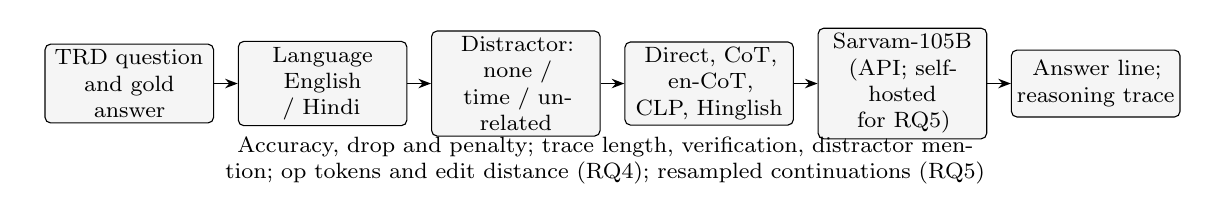
\begin{tikzpicture}[
  box/.style={draw, rounded corners=2pt, align=center, font=\footnotesize, minimum height=0.85cm, text width=2.0cm, inner sep=2pt, fill=gray!8},
  arr/.style={-{Stealth[length=1.6mm]}, semithick}, node distance=0.3cm]
\node[box] (q) {TRD question\\and gold answer};
\node[box, right=of q] (l) {Language\\English / Hindi};
\node[box, right=of l] (d) {Distractor: none /\\time / unrelated};
\node[box, right=of d] (p) {Direct, CoT, en-CoT,\\CLP, Hinglish};
\node[box, right=of p] (m) {Sarvam-105B\\(API; self-hosted\\for RQ5)};
\node[box, right=of m] (o) {Answer line;\\reasoning trace};
\draw[arr] (q) -- (l); \draw[arr] (l) -- (d); \draw[arr] (d) -- (p); \draw[arr] (p) -- (m); \draw[arr] (m) -- (o);
\node[font=\footnotesize, align=center, text width=14.4cm, below=0.12cm of o.south east, anchor=north east] {Accuracy, drop and penalty; trace length, verification, distractor mention; op tokens and edit distance (RQ4); resampled continuations (RQ5)};
\end{tikzpicture}

\vspace{4pt}
\footnotesize
\begin{tabularx}{\textwidth}{@{}X@{}}
\textbf{English:} Today is 2027-05-16, and I have a recurrence every 13 days. Without counting today, what is the date of the 7 occurrence? \textbf{Gold:} 2027-08-15.\\
\textbf{Hindi:} \hi{आज 2027-05-16 है, और मेरे पास हर 13 दिनों पर एक पुनरावृत्ति है। आज को छोड़कर, 7वीं आवृत्ति की तिथि क्या है?}\\
\textbf{Time-related distractor, prepended:} The last time I had a weekly commitment was in January. / \hi{आखिरी साप्ताहिक प्रतिबद्धता जनवरी में थी।}\\
\end{tabularx}

\vspace{2pt}
\scriptsize\setlength{\tabcolsep}{3.5pt}
\begin{tabular}{@{}llll@{\hspace{1em}}llll@{}}
\toprule
Condition & Reasons in & No distractor & Time-related & Condition & Reasons in & No distractor & Time-related \\
\midrule
English direct & -- & 2027-06-05 \no & 2027-04-19 \no & en-CoT (Hindi Q.) & English & 2027-08-15 \ok & cut off at limit \\
English CoT & English & 2027-08-15 \ok & cut off at limit & CLP (Hindi Q.) & English & 2027-08-02 \no & 2027-08-02 \no \\
Hindi direct & -- & 2027-07-27 \no & 2027-03-06 \no & Hinglish (English Q.) & Roman mix & 2027-08-02 \no & 2027-08-01 \no \\
Hindi CoT & Hindi & 2027-08-02 \no & 2027-04-20 \no & Hinglish (Hindi Q.) & Devanagari mix & 2027-08-02 \no & 2027-07-06 \no \\
\bottomrule
\end{tabular}
\caption{The pipeline, with real responses to one question (long, date recurrence, ID 12). This item was picked to illustrate the design, not as a typical case. The answer 2027-08-02 adds six intervals where seven are needed; the Hindi CoT and CLP traces do so by counting today as the first occurrence. With the distractor, Hindi CoT writes \hi{जनवरी 2027 की आखिरी तारीख (31 जनवरी 2027) ही हमारी शुरुआती तारीख है} (``the last date of January 2027 (31 January 2027) is our start date''), and English CoT and en-CoT keep trying to fit January into the question until the token limit. Cut-offs count as wrong only under strict scoring.}
\label{fig:design}
\end{figure*}

\paragraph{Measures.}
\emph{Answered} accuracy drops responses with no answer line, which is what our figures show. \emph{Strict} accuracy counts them as wrong and is closer to TRD's own scoring \citep{mazzia-etal-2026-benchmarking}. Answered-only flatters English CoT, which has the most cut-offs among thinking-off conditions, so we give both for headlines and flag conclusions that change. The \emph{drop} is accuracy without a distractor minus accuracy with one, and the \emph{penalty} is the CoT drop minus the direct drop. For traces, we record length, a verification phrase regex and distractor mentions against a placebo measured on the same question without the distractor.

For RQ4 a regex parser turns each trace into operation tokens with operands, such as \texttt{SUB 2025-05-26 4}. The reasoning divergence score (RDS) is their Levenshtein distance \citep{levenshtein1966binary} divided by the longer length. A substitution between a partial and a full date costs 0.5, a rule whose effect we confirmed is negligible. The length floor, $|n-m|/\max(n,m)$, is the lowest RDS two lengths allow, and RDS equals floor plus $(1-\text{floor})$ times a floor-adjusted score. Coverage is 95--96\% of CoT segments on standard content and 86--88\% on thinking-mode reasoning. A sample of 240 tokens read by one LLM annotator, not validated by a person, puts precision at 85\% for the operation and 77\% with its arguments.

\paragraph{Statistics.}
Accuracy intervals are 95\% cluster bootstraps over questions, since a question appears in three distractor conditions \citep{berg-kirkpatrick-etal-2012-empirical}. RQ4 odds ratios use question-clustered standard errors, and task-by-level statements use uncorrected intervals. Task-level tests use exact McNemar with Holm correction over nine tasks \citep{mcnemar-1947-note,holm-1979-simple,dror-etal-2018-hitchhikers}, and mention associations use Mantel-Haenszel odds ratios \citep{mantel-haenszel-1959-statistical}. These intervals treat sentences and prompts as fixed, so they understate uncertainty about other wordings.

\section{Results}
\label{sec:results}

\begin{table*}[t]
\centering
\small
\begin{tabular}{@{}lrrrrrrrr@{}}
\toprule
& \multicolumn{2}{c}{English Q.} & \multicolumn{4}{c}{Hindi Q.} & \multicolumn{2}{c}{Hinglish prompt} \\
\cmidrule(lr){2-3}\cmidrule(lr){4-7}\cmidrule(l){8-9}
& Direct & CoT & Direct & CoT & CLP & en-CoT & English Q. & Hindi Q. \\
\midrule
Date addition & 85.6 & 98.0 & 82.8 & 85.1 & 92.7 & 95.7 & 87.3 & 85.9 \\
Date subtraction & 86.0 & 95.2 & 84.8 & 66.0 & 86.9 & 94.0 & 70.7 & 71.0 \\
Date duration & 84.0 & 99.3 & 78.9 & 88.3 & 92.7 & 97.7 & 92.9 & 82.8 \\
Date recurrence & 22.1 & 90.3 & 2.8 & 20.1 & 27.0 & 70.3 & 53.8 & 18.9 \\
Day of week & 14.9 & 69.5 & 15.2 & 21.0 & 31.8 & 52.5 & 34.7 & 23.5 \\
Interval date & 43.2 & 50.7 & 46.8 & 23.9 & 35.3 & 44.1 & 38.5 & 23.6 \\
Time addition & 70.5 & 95.9 & 75.6 & 73.5 & 88.2 & 92.6 & 82.9 & 72.3 \\
Time subtraction & 64.7 & 97.7 & 64.9 & 75.2 & 90.1 & 95.7 & 85.3 & 74.2 \\
Time duration & 65.7 & 98.9 & 44.7 & 80.1 & 86.7 & 98.1 & 90.0 & 80.9 \\
\midrule
Short & 77.8 & 93.2 & 73.9 & 69.5 & 77.2 & 83.0 & 82.9 & 66.5 \\
Medium & 69.6 & 91.6 & 65.3 & 65.4 & 75.7 & 84.9 & 78.8 & 67.4 \\
Long & 61.2 & 89.3 & 57.9 & 60.4 & 71.3 & 84.4 & 70.4 & 60.9 \\
Very long & 54.3 & 87.2 & 48.4 & 53.7 & 65.8 & 83.5 & 64.0 & 53.7 \\
Very very long & 35.5 & 82.9 & 30.3 & 47.9 & 61.5 & 78.5 & 58.2 & 48.3 \\
\midrule
No distractor & 60.6 & 89.3 & 56.0 & 60.2 & 69.3 & 84.1 & 70.6 & 61.0 \\
Time-related & 59.9 & 88.1 & 54.9 & 58.9 & 69.3 & 81.0 & 69.7 & 59.1 \\
Unrelated & 58.6 & 89.2 & 54.6 & 59.1 & 72.3 & 83.6 & 72.4 & 58.0 \\
\midrule
\textbf{All, answered} & 59.7 & 88.9 & 55.2 & 59.4 & 70.3 & 82.9 & 70.9 & 59.4 \\
\textbf{All, strict} & 59.6 & 86.0 & 55.2 & 59.0 & 69.9 & 80.8 & 70.3 & 59.1 \\
\bottomrule
\end{tabular}

\caption{Answered accuracy (\%) on the same 2,250 questions, by task, level and distractor condition. The last row counts unanswered responses as wrong.}
\label{tab:accuracy}
\end{table*}

\subsection{RQ1: CoT helps English far more than Hindi}

Over all 6,750 questions, CoT raises English accuracy by 29.5 points and Hindi by 4.7 (Table~\ref{tab:baseline}). The English-Hindi gap goes from 4.2 points under direct answering to 29.1 under CoT (strict 4.2 and 26.7), and it holds in each distractor condition, so pooling does not create it. With no distractor at all, Hindi CoT lowers accuracy on date subtraction by 19.9 points [16.4, 23.4] and on interval date by 23.3 [19.0, 27.7], and both stay significantly negative with either distractor. English CoT is never significantly below direct in any task or task-by-level cell.

\begin{table}[t]
\centering
\footnotesize
\setlength{\tabcolsep}{3pt}
\begin{tabular}{@{}lrrrr@{}}
\toprule
& Direct & CoT & Gain [95\% CI] & Strict \\
\midrule
English & 59.0 & 88.5 & +29.5 [28.5, 30.6] & +26.8 \\
Hindi & 54.7 & 59.4 & +4.7 [3.6, 5.7] & +4.2 \\
\midrule
By distractor & \multicolumn{2}{c}{None} & Time-related & Unrelated \\
English & \multicolumn{2}{c}{+28.8} & +29.1 & +30.7 \\
Hindi & \multicolumn{2}{c}{+5.6} & +3.4 & +5.0 \\
Gap under CoT & \multicolumn{2}{c}{+28.0} & +29.7 & +29.7 \\
Gap, direct & \multicolumn{2}{c}{+4.8} & +4.0 & +3.9 \\
\bottomrule
\end{tabular}

\caption{CoT gain on all 6,750 questions, in points. All values are answered except the Strict column, which counts unanswered as wrong. By-distractor English and Hindi rows are gains.}
\label{tab:baseline}
\end{table}

Two pooled results do not survive a split. The time duration gain gap (English gain minus Hindi gain), +2.3 pooled, is $-$5.2 with no distractor, +14.5 with a time-related one and $-$2.2 with an unrelated one (only +14.5 is significant), and Hindi CoT's harm at the short level ($-$4.3 pooled) comes from the distractor conditions ($-$1.9 [$-$4.5, 0.7] without one, $-$6.2 and $-$4.7 with). The gap under CoT widens with difficulty in points, from 24.0 to 34.9 (strict 23.0 to 31.1), but a logistic trend is not significant (OR 0.97 per level, $p=0.21$), so we describe the widening only on the points scale.

\subsection{RQ2: Distractor effects are small and depend on the sentence}

A time-related distractor costs Hindi CoT 2.6 points [1.3, 3.8], which is 2.2 more than it costs Hindi direct answers (penalty [0.6, 3.8]). Removing any single sentence leaves the penalty between 1.8 and 2.6. We withdraw our mid-report claim that distractors make CoT fragile only in Hindi. For time-related sentences, the Hindi-minus-English penalty is +2.6 [0.4, 4.7] answered, but +1.4 [$-$0.7, 3.5] strict, as English CoT's drop grows from 0.9 to 2.2 [1.3, 3.2]; it is not significant on logit specifications unless recurrence is removed. With unrelated sentences it is +2.6 [0.5, 4.6] answered and +2.8 [0.8, 4.8] strict, but because English CoT resists a fall in English direct answers: the Hindi penalty is null (+0.7). Treating the 45 task-sentence units as the sample gives a mean Hindi penalty of +2.3 [$-$0.1, 4.6], so the penalty may not extend to new sentences.

The largest effect, found post hoc among 90 sentences, comes from one sentence, the one in Figure~\ref{fig:design}. It sends 92 of 134 English CoT traces to the token limit (4 of 134 without it) and cuts strict English accuracy on those questions from 88.8\% to 19.4\%. Hindi has no cut-offs, but falls from 26.9\% to 2.2\%. None of the 92 traces is a verbatim loop. In a systematic sample of 23, read from excerpts by one LLM annotator, 18 mainly search for a January start date until the budget ends. This sentence competes with the premise of the question, so it is not irrelevant in the GSM-IC sense. Removing it takes the Hindi recurrence penalty from +4.5 to +0.3 [$-$4.6, 4.9]; English stays at +8.5 (strict +9.9).

Hindi traces mention distractors more often than English ones (25.0\% vs 8.5\% for time-related sentences, with near-zero placebo on a stricter word list chosen after seeing the data). On this list, mentions of time-related sentences go with lower accuracy (Hindi OR 0.77 [0.67, 0.89], English 0.57 [0.38, 0.85]); on the original list English is 0.92, and unrelated sentences show no such link (1.15, 1.30). RQ5 tests the association directly.

\subsection{RQ3: The gap follows the language of reasoning}

\begin{figure}[t]
\centering
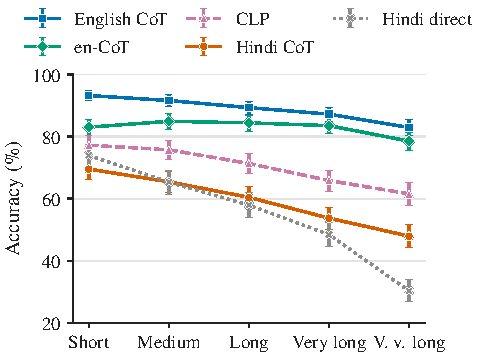
\includegraphics[width=\columnwidth]{by_level}
\caption{Answered accuracy by difficulty on 2,250 questions, with 95\% bootstrap intervals.}
\label{fig:level}
\end{figure}

Table~\ref{tab:accuracy} gives all conditions on the same questions, and Figure~\ref{fig:level} five of them. Asking for English reasoning on Hindi questions reaches 82.9\%, against 59.4\% for Hindi CoT and 88.9\% for English questions with English CoT. Of the 29.5-point gap [28.1, 30.9], 23.5 [22.1, 24.9] separates en-CoT from Hindi CoT with the question fixed, and 6.0 [5.0, 7.1] remains between the question languages (Figure~\ref{fig:decomposition}). That is 79.7\% [76.4, 82.9] of the gap, or 80.7\% under strict scoring, and 22.0 to 24.5 points in each distractor condition. The reasoning part exceeds the question part on every task, and at every level except short, where the two are not distinguishable. The direct-answer gap, which involves no reasoning, is 4.5 [3.3, 5.8], close to the 6.0.

\begin{figure}[t]
\centering
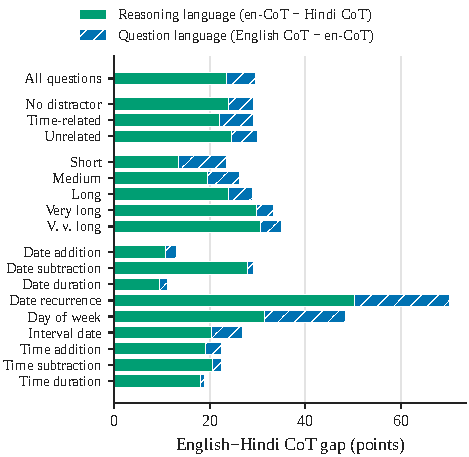
\includegraphics[width=\columnwidth]{decomposition}
\caption{The English-Hindi CoT gap on 2,250 questions, split on one path through three conditions. No condition pairs English questions with Hindi reasoning, so the split is descriptive.}
\label{fig:decomposition}
\end{figure}

Trace structure splits the same way (Figure~\ref{fig:distance}). Edit distance between English CoT and en-CoT traces, which share a reasoning language, is 0.730, close to the 0.713 between English traces of one question with and without a distractor. Between en-CoT and Hindi CoT traces on identical Hindi questions it is 0.837, close to the 0.853 between English and Hindi CoT. Verification follows too: 86.1\% of English CoT traces contain a verification phrase, against 74.2\% for en-CoT and 1.3\% for Hindi CoT. A g-formula estimate within task and level attributes 1.0\% [$-$6.3, 9.0] of the en-CoT gain to it, while it is associated with much of the day-of-week residual to English (63.6\% [39.8, 97.0]). Both estimates are observational.

\begin{figure}[t]
\centering
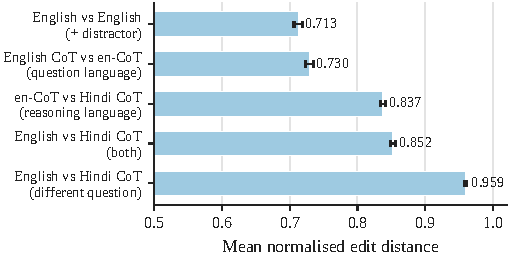
\includegraphics[width=\columnwidth]{distance}
\caption{Mean RDS between trace pairs on 2,250 questions, including English traces with and without a distractor and English-Hindi pairs from different questions, with 95\% intervals.}
\label{fig:distance}
\end{figure}

\paragraph{CLP.}
CLP scores 70.3\%, which is 10.9 points [9.6, 12.2] above Hindi CoT and holds in each distractor condition (+9.0, +10.4, +13.3). It beats Hindi direct by 15.1 [13.5, 16.7] overall, but is significantly worse on interval date (35.3\% vs 46.8\%). en-CoT beats CLP by 12.6 [11.4, 13.9], which reverses the order \citet{qin-etal-2023-cross} report for GPT-3.5 on MGSM, where CLP scores 70.6 and En-CoT 57.8; model, task and settings all differ. Carry-over from the first turn is one candidate, though stage 1 was not randomised. On the three date-answer tasks, stage 2 is right in 97.5\% of responses when stage 1 ends at the gold date and in 20.1\% when it does not. Within the same question the difference is +62.5 points [57.1, 68.0], while the same split on en-CoT differs by about 7. \citeauthor{qin-etal-2023-cross} also note that stage 1 may give preliminary answers, so we add only its size here. Our temperature of 0 and added language rule may contribute, and we did not test this.

\paragraph{Hinglish.}
Prompting for Hinglish costs English questions 18.0 points [16.8, 19.2] (strict 15.7), on all nine tasks and in each distractor condition. Hindi questions do not change on average ($-$0.0 [$-$1.3, 1.2]), so the gap narrows only because English falls. Task effects cancel inside that mean: date duration falls by 5.5 points and date subtraction rises by 5.1. The model largely ignores the script instruction on Hindi questions, where 68.5\% of traces have a Devanagari majority and 25.5\% have no Devanagari, so this arm mostly tests code-mixed Devanagari.

The English loss also appears without Hindi function words. Those traces still lose 10.3 points [8.3, 12.3], and verification on those traces falls from 86.5\% to 18.6\%. Traces with Hindi function words lose 11.3 points more [9.0, 13.6] within task, level and distractor (8.4 to 12.0 across 48 threshold pairs), on all nine tasks at each, but the model chooses the style, so this is an association. On Hindi questions Roman traces do no better than Devanagari ones ($-$2.8 [$-$5.2, $-$0.5]; $-$2.3 [$-$5.0, 0.4] within question). One failure is shared: English date subtraction crossing a month boundary falls from 90.1\% to 42.3\%, near Hindi CoT's 36.2\%, while same-month questions stay at 97.4\%.

\paragraph{Where English reasoning does not help.}
Backward answers on date recurrence are concentrated at $k=1$ (en-CoT 67.1\%, Hindi CoT 67.8\%, CLP 69.0\%, English CoT 3.5\%), and they do not respond to the reasoning language (Appendix, Figure~\ref{fig:recurrence}). The Hindi carrier ``\hi{आज को छोड़कर, 1वीं आवृत्ति}'' is a candidate source, since \hi{1वीं} is non-standard. But equally non-standard ordinals at $k=2$ to 4 give almost none (2 of 229 for en-CoT), and we did not rerun a corrected template, so this remains unresolved. Removing $k=1$ moves en-CoT's pooled gap to English only from 6.0 to 5.3. en-CoT's gap to English narrows from 10.2 points at short to 4.3 at very very long, but this depends on recurrence: without $k\le 2$ the change is +0.8 [$-$2.5, 4.1].

\paragraph{Thinking mode.}
With thinking on, Hindi CoT reaches 97.9\% answered and 89.9\% strict, and its hidden reasoning is 79\% English words. This fits the account above but cannot confirm it, because thinking and a fourfold token budget change together; at a simulated 4,096 limit, strict Hindi CoT would be 43.8\%, below the 59.9\% with thinking off. Within these traces a higher English share does not predict higher accuracy.

\subsection{RQ4: Divergence is mostly built into the metric}

On 20,662 answered pairs, English and Hindi disagree on 31.4\%, and a logistic regression finds an odds ratio of 4.92 per 0.1 RDS [4.58, 5.30], controlling for task, difficulty, distractor and mode. This says little about reasoning, because RDS contains final-answer tokens and the outcome depends on the answers. Replacing only Hindi's answer values in the 11,309 both-correct thinking-off pairs raises mean RDS by 0.082, which is 68\% of the 0.120 gap to disagreeing pairs.

\begin{figure}[t]
\centering
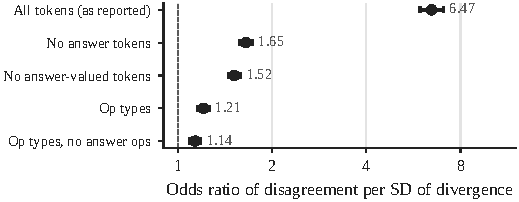
\includegraphics[width=\columnwidth]{lr_forest}
\caption{Odds ratio of disagreement per SD of divergence, under task, difficulty, distractor and mode controls on 20,648 pairs, with SEs clustered by question.}
\label{fig:lrforest}
\end{figure}

Removing answer tokens drops the odds ratio per SD from 6.47 to 1.65, and op types without answer ops give 1.14, or 1.21 with them (Figure~\ref{fig:lrforest}). The fall appears in each distractor condition (OR per 0.1: 5.37, 4.60, 4.95 to 1.13, 1.08, 1.09). Out of fold, op-type divergence adds 0.0007 AUC [$-$0.0004, 0.0018] beyond the controls, and within a question it barely separates disagreeing from agreeing variants (concordance 0.516 [0.501, 0.530]). A within-question slope survives Holm correction only for date recurrence (OR per 0.1, 1.42 [1.25, 1.61]) and day of week (1.26 [1.11, 1.43]). Simply comparing the two final answers gives AUC 0.951. RDS is also joint highest on both-wrong pairs (0.925, as Hindi-only), which count as agreement, so it tracks whether a trace failed more closely than whether the languages disagree.

We cannot conclude from this that failing traces follow the same route. Op types separate a different question from the same question by only +0.012, and within Hindi, wrong and right traces on one question do differ (+0.030 [0.021, 0.039]).

The choice of normalisation changes one conclusion. The floor is 58--61\% of mean RDS on standard content and on thinking-mode reasoning. Raw RDS does not separate the two on matched questions (+0.005 [$-$0.002, 0.011]), but the floor-adjusted score does (+0.088 [0.072, 0.105]), so we report both parts. The thinking-on and thinking-off comparison is confounded as well: counting unanswered as wrong on the same 450 questions, disagreement is 10.9\% against 31.7\% (OR 0.23 [0.18, 0.30]), with thinking and budget changing together.

\subsection{RQ5: Distractor mentions under intervention}

\paragraph{Setup.}
From the CoT responses with the time-related distractor, we keep wrong answers whose trace mentions it before answering: 526 Hindi and 37 English. The API cannot continue a partial reply, so we served an FP8 build of the model with vLLM. Agreement with the API on 90 calibration questions is $-$2.2 points [$-$13.3, 7.8], which does not establish that they are the same, and on 22 English questions the self-hosted model scored 24.7 points lower, and on 278 Hindi questions 5.7 higher [0.5, 10.8]. We therefore make no causal claim for English.

\paragraph{Deleting mentions.}
Deleting the mentioning sentence, against deleting a neutral sentence, shows no detectable benefit on the 222 Hindi traces with a matching neutral sentence (+0.0 [$-$6.8, 7.2] greedy, +4.5 [$-$2.7, 11.7] sampling). With one continuation per version this had about 24\% power for a 5-point effect, so it does not show that deletion has no effect.

\paragraph{Resampling.}
Following \citet{bogdan-etal-2025-anchors} and \citet{macar-etal-2026-branches}, we let $k$ be the first sentence mentioning the distractor and resample seven times per trace at temperature 0.8. Arm \emph{P} continues from before $k$ on the same question, \emph{Q} does so with the distractor removed from the question, \emph{M} continues from after $k$, and \emph{P1} from one sentence earlier. The design was written down before the run according to our notes, but it was first committed afterwards and followed the deletion experiment on 234 of the same traces, and the study was not publicly registered.

\begin{figure}[t]
\centering
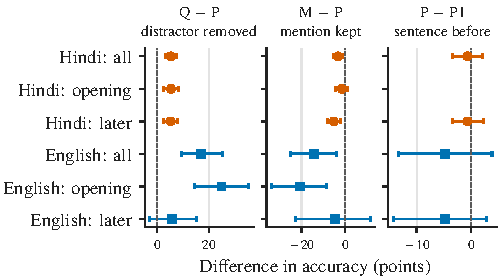
\includegraphics[width=\columnwidth]{interventions}
\caption{Resampling contrasts with 95\% intervals. Traces were selected for being wrong, the distractor is time-related, and unanswered continuations count as wrong. P$-$P1 uses only traces with $k\ge1$. English is descriptive.}
\label{fig:interventions}
\end{figure}

In Hindi, Q is 45.2\% and P is 40.0\%, a difference of +5.3 [3.2, 7.4] (Figure~\ref{fig:interventions}). The distractor thus accounts for a net 8.8\% [5.5, 12.1] of errors arising from that point, a lower bound on how often it was necessary \citep{tian-pearl-2000-probabilities}, and most continuations wrong with it are also wrong without it. The interval widens to [$-$0.3, 9.4] when the 29 sentences are resampled, and one sentence, from Figure~\ref{fig:design}, supplies 58\% of the summed effect (without it, +2.8 [0.4, 5.0]). Keeping the sentence with the first mention lowers accuracy by 3.3 points [1.2, 5.4], but on the 248 traces with $k\ge1$, the test of whether it exceeds the preceding sentence, (M$-$P)$-$(P$-$P1), is not significant ($-$4.6 [$-$9.6, 0.6], $p=0.09$; P$-$P1 $-$0.7 [$-$3.5, 2.1]), so it cannot be told apart from one more step along a trace that ended wrong.

Our design cannot separate the distractor in the question from the act of writing it, because free continuations mention it in 57.8\% of rollouts. In later-mention traces, rollouts with no mention match the no-distractor arm (+0.0 [$-$4.8, 4.7]) and those with a mention do not (+8.7 [3.7, 13.6]); these subgroups are post-treatment. Unanswered Hindi rollouts rise from 5.7\% to 10.0\%, but on the API Hindi non-completion barely moves (0.81\% to 0.89\%), so this may belong to the self-hosted setting.

\section{Discussion}
\label{sec:discussion}

Across accuracy, trace distance and verification, the instructed language of reasoning goes with more of the gap than the language of the question. This fits the direct-answer gap and prior work favouring English reasoning \citep{shi-etal-2023-mgsm,yong2025crosslingual,qi-etal-2025-models}. On this model and these tasks, requesting English reasoning on Hindi questions scored higher; we did not test replying to users in Hindi. The en-CoT gain here is far larger than MGSM's, which may reflect zero-shot prompting, the task or the model.

A method's ranking may not transfer between models and tasks: a single English turn beat two turns here, and carry-over from stage 1 is a candidate explanation. A Hinglish reasoning instruction can also backfire, as it made English questions worse, partly without any Hindi in the trace. Those traces verified far less often, but the model chooses to verify, and adjustments for it disagree, so we do not treat it as the mechanism.

A trace metric that includes outcome-bearing tokens can look predictive of that outcome, so a large odds ratio needs a view that removes those tokens and a baseline for resolution before it can be read. Reading a wrong trace that mentions a distractor can also mislead, since most such errors recur without the distractor.

\section{Conclusion}
\label{sec:conclusion}

On Sarvam-105B and TRD, CoT widens the English-Hindi gap from about 4 points to about 29. Most of that gap closes when the same Hindi questions are reasoned through in English, some of it with CLP, and on average none through a Hinglish prompt on Hindi questions, whose traces stayed mostly Devanagari. Divergence between traces predicts disagreement far more weakly without answer tokens, and op types add almost nothing. The average distractor effect is small and varies by sentence, and our design cannot separate it from the model's mention of them.

\section{Limitations and Future Work}
\label{sec:limitations}

\paragraph{Scope.} Everything here concerns one model, greedy decoding except in the resampling arms, one prompt per condition, one dataset seed and two languages. Intervals cover question sampling only, so they say nothing about other wordings, and with temperature 0 there is no sampling noise estimate for the main runs.

\paragraph{Identification.} Language and prompt wording are confounded in every comparison across prompting conditions, including our decomposition. No condition pairs English questions with Hindi reasoning, so the split is one path and depends on its order. Trace style, mentions and verification are chosen by the model or measured after it responds, so they support association only. Runs span about a month, the provider changed its API responses in that time, and condition and run date are partly confounded.

\paragraph{Data.} The added conditions use the first 50 of 150 questions per cell. This subset is too small for distractor contrasts of a few points. Hindi distractors are not literal translations, and some Hindi carriers are awkward, so English-Hindi distractor comparisons are not strictly parallel. Distractor sentences are a fixed pool assigned unevenly across tasks, and the generator's seed reset makes levels share sentence mixes. TRD's time-task offsets in the code differ from the difficulty ranges its paper lists.

\paragraph{Measurement.} The parser is regex-based and imperfect. Mention and verification rules are lexical. All our hand-labelled samples were read by a single LLM annotator without blinding or human validation, including parser precision and our review of the Hindi templates; they should be checked by people.

\paragraph{Interventions.} Resampling covers only originally wrong traces and time-related distractors, on a quantised self-hosted model at a different temperature from the source traces. We did not test whether mentions harm traces that would otherwise be correct.

\paragraph{Thinking mode.} This pilot has 10 questions per cell and a fourfold budget, and it changes thinking and budget together.

\paragraph{Future work.} The most informative next steps are: rerunning recurrence with corrected Hindi carriers; adding English questions with Hindi reasoning to complete the design; an English CoT prompt without the language lock and several paraphrases of each prompt; CLP with solving forbidden in stage 1; thinking on and off at equal budgets; a question-by-mention factorial on both correct and wrong traces; and human annotation of the labelled samples.

\bibliography{references}

\clearpage
\appendix
\section*{Appendix A. Worked Examples}
\addcontentsline{toc}{section}{Appendix A. Worked Examples}

\footnotesize
\noindent\textbf{Hinglish, English question, wrong.} Date subtraction, short. ``Today is 2025-05-01, what was the date 3 days ago?'' Gold 2025-04-28. Standard English CoT answered correctly. Excerpt: \emph{Step 4: 01 minus 3 karne par hum 31 April par aayenge. Step 5: Isliye, 3 days ago ki date 2025-04-30 thi.} Answer: 2025-04-30.

\smallskip
\noindent\textbf{en-CoT, $k=1$, backward answer.} Date recurrence, short, ID 5, time-related distractor, Hindi question with \hi{आज को छोड़कर, 1वीं आवृत्ति}. Excerpt: \emph{Given the phrasing ``excluding today,'' this suggests we need to find what comes before.} Answer: 2025-04-06. Gold 2025-04-14.

\smallskip
\noindent\textbf{CLP, stage 1 anchors stage 2.} Date recurrence, long, ID 12, no distractor. Stage 1 ends: \emph{Therefore, the date of the 7th occurrence is 2 August 2027.} Stage 2 ends: \emph{Adding 78 days to 16 May 2027 also results in 2 August 2027.} Answer: 2027-08-02. Gold 2027-08-15.

\smallskip
\noindent\textbf{Resampling arms.} Date recurrence, long, ID 12, Hindi, time-related distractor. The original trace answered 2027-04-20. Correct continuations out of seven: Q 5, P 2, M 0, P1 2. A single example cannot show an effect; Figure~\ref{fig:interventions} gives the aggregates.

\normalsize
\section*{Appendix B. Secondary Figures}
\addcontentsline{toc}{section}{Appendix B. Secondary Figures}

\begin{figure}[!ht]
\centering
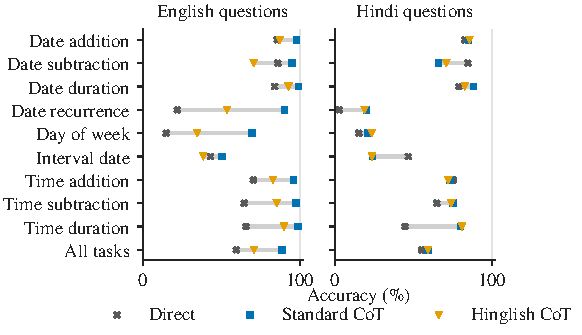
\includegraphics[width=\columnwidth]{hinglish_tasks}
\caption{Accuracy by task under the Hinglish prompt, answered.}
\label{fig:hingtasks}
\end{figure}

\begin{figure}[!ht]
\centering
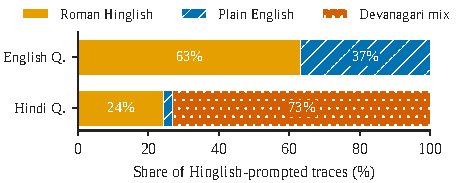
\includegraphics[width=\columnwidth]{hinglish_style}
\caption{Script style of Hinglish-prompted traces.}
\label{fig:hingstyle}
\end{figure}

\begin{figure}[!ht]
\centering
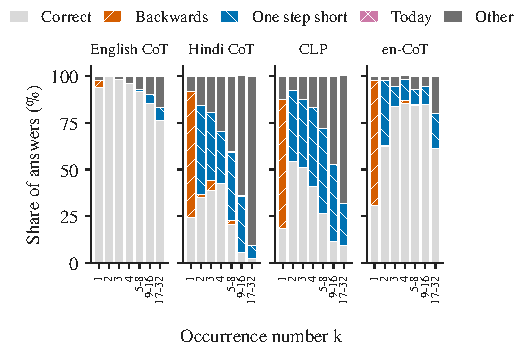
\includegraphics[width=\columnwidth]{recurrence_k}
\caption{Date recurrence answers by occurrence number $k$, on 2,250 questions. Backward answers concentrate at $k=1$ under every prompt on Hindi questions; one-step-short answers run through every $k$.}
\label{fig:recurrence}
\end{figure}

\begin{figure}[!ht]
\centering
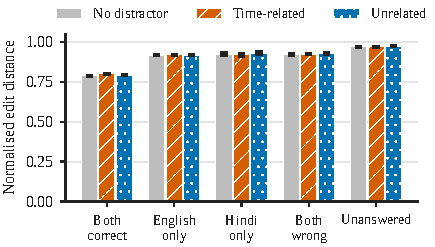
\includegraphics[width=\columnwidth]{ed_outcome}
\caption{Mean RDS by correctness outcome and distractor condition. Failure outcomes sit about 0.13 above both-correct.}
\label{fig:edoutcome}
\end{figure}

\begin{figure}[!ht]
\centering
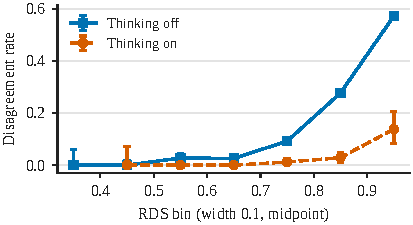
\includegraphics[width=\columnwidth]{lr_bins}
\caption{Observed disagreement rate by RDS bin. Answer tokens are included, so this rise is largely mechanical.}
\label{fig:lrbins}
\end{figure}

\begin{figure*}[t]
\centering
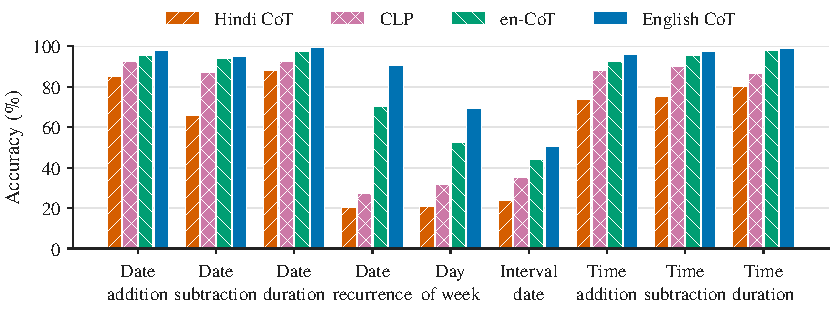
\includegraphics[width=0.92\textwidth]{task_bars}
\caption{Answered accuracy by task on 2,250 questions.}
\label{fig:taskbars}
\end{figure*}

\begin{figure*}[t]
\centering
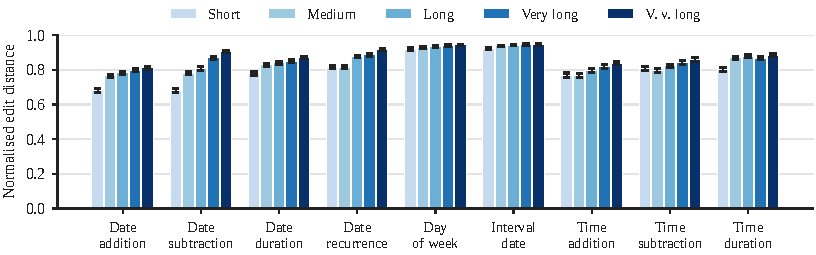
\includegraphics[width=0.92\textwidth]{ed_task_difficulty}
\caption{Mean RDS by task and difficulty, standard and thinking-on visible replies pooled, error bars treating pairs as independent. Means sit near the ceiling on day of week and interval date, so RDS cannot track difficulty there.}
\label{fig:edtask}
\end{figure*}


\end{document}
